% !TEX encoding = UTF-8
% !TEX TS-program = pdflatex
% !TEX root = ../tesi.tex

%**************************************************************
\chapter{Progettazione}
\label{cap:progettazione}
\label{sec:tecnologie-strumenti}

In questo capitolo vengono illustrate le strategie di progettazione adottate per la realizzazione del prodotto in questione. La progettazione viene descritta ad alto livello senza descrivere in dettaglio tutti i diagrammi delle classi. 

\section{Progettazione Frontend}
\label{sec:progettazione}
Come prima cosa sono stati realizzati utilizzando Figma i prototipi delle pagine da creare. In questo modo è stato possibile capire sin da subito la struttura delle pagine, rendendo cosi molto semplice la progettazione architetturale di tale pagine.
\subsection{Pagina cotenente l'editor}
Questa pagina contiene l'editor \emph{drag and drop}. Per creare la struttura di questa pagina sono stati studiati diversi editor online che forniscono le stesse funzionalità(in diversi contesti). Dopo una attenta analisi delle strutture dei diversi editor online è stato concepita la seguente struttura:
\begin{figure}[!h] 
	\centering 
	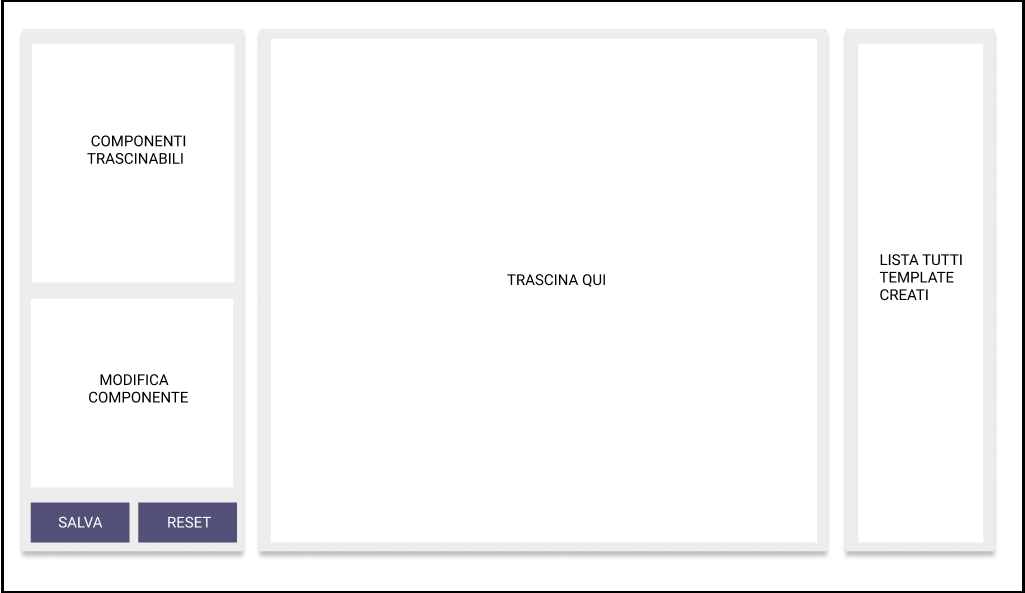
\includegraphics[width=0.9\columnwidth]{mock/mockeditor} 
	\caption{Mock pagina contenente l'editor}
\end{figure}  
\\
\begin{itemize}
	\item Il primo contenitore in alto a sinistra dovrà contenere tutti i componenti trascinabili. Ogni elemento rappresenta uno specifico tipo di oggetto HTML e CSS, come ad esempio il testo, banner, titolo, immagine ecc;
	\item Il secondo contenitore a sinistra contiene tutte le proprietà modificabili per ogni elemento;
	\item Il contenitore in centro(container) rappresenta la zona dove tutti gli elementi vengono trascinati. In questo contenitore viene visualizzato a schermo il contenuto HTML e CSS di ogni elemento trascinato. Inoltre dovrà essere possibile modificare tale contenuto ed eliminare un elemento se necessario;
	\item Il contenitore a destra dovrà contenere tutti i template realizzati dagli utenti. Quindi esso contiene semplicemente una lista di tutti i template.  
\end{itemize}

\subsection{Pagina contenente il widget} Questa pagina contiene una semplice lista che dovrà contenere tutti i template da visualizzare nella pagina dei \emph{tickets}, in modo che essi posono essere scelti dagli agenti di Zendesk.
\\ 
\subsection{Pagina login}
Semplice pagina contenete il \emph{form} per il login. Una volta inseriti i valori validi l'utente sarà utenticato come amministratore, caricandoli cosi la pagina degli amministratori. 
\begin{figure}[!h] 
	\centering 
	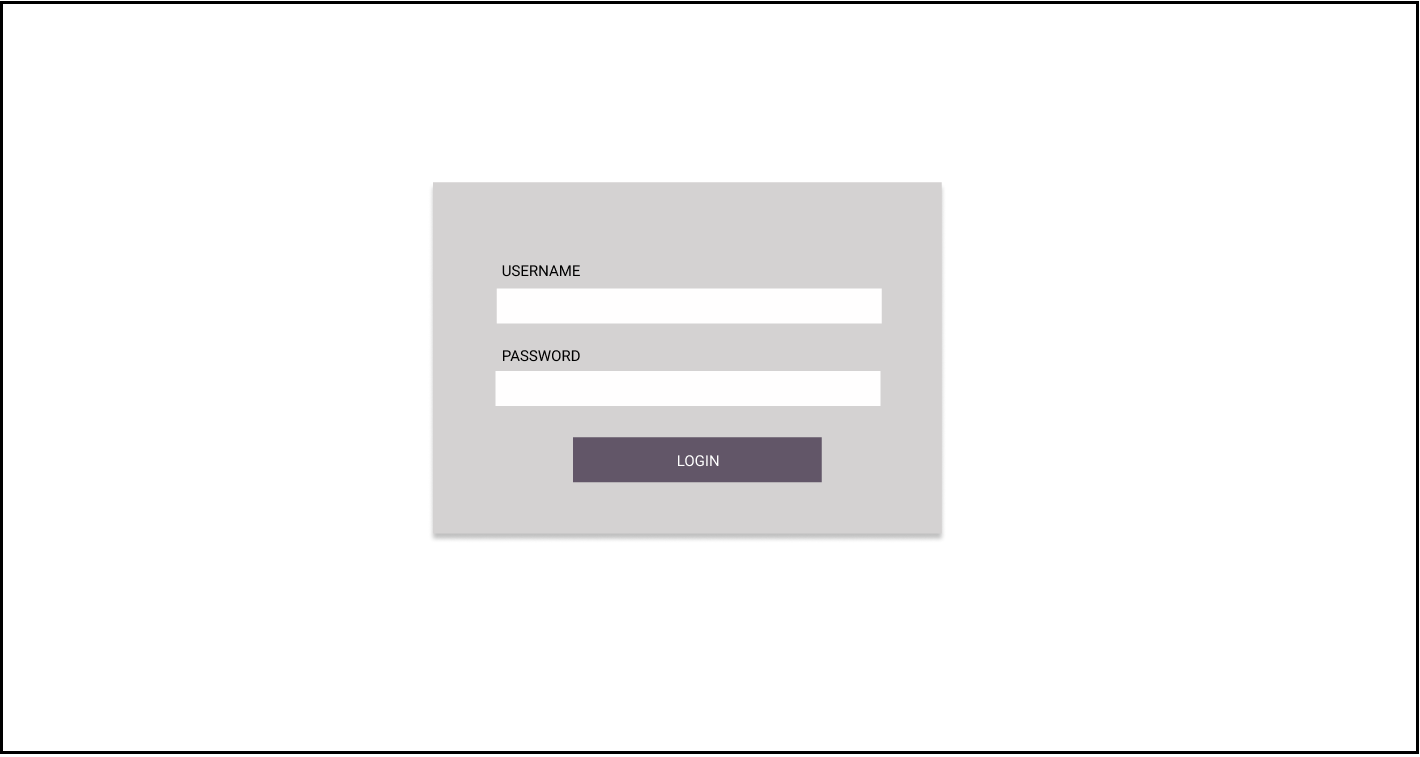
\includegraphics[width=1\columnwidth]{mock/mocklogin} 
	\caption{Mock pagina di login}
\end{figure}  \newpage
\subsection{Pagina degli amministratori}
Questa pagina dovrà essere realizzata per gli amministratori di Nextep, per permettere a loro di gestire tutti i clienti utilizzatori dell'applicazione. 
\begin{figure}[!h] 
	\centering 
	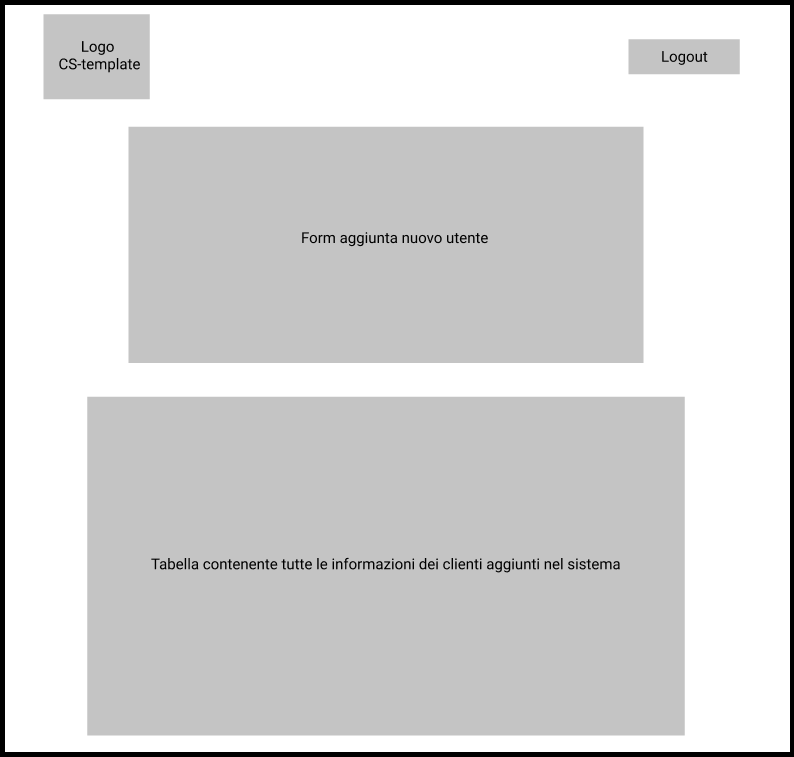
\includegraphics[width=0.8\columnwidth]{mock/mockadmin} 
	\caption{Mock pagina degli amministratori}
\end{figure} 
\newpage 
\begin{itemize}
	\item Contiene un semplice form per aggiungere un nuovo cliente;
	\item Contiene una semplice tabella, dove ogni elemento della tabella contiene le informazioni di un singolo cliente.
\end{itemize}
\subsection{Struttura applicazione}
Essendo un'unica applicazione che contiene sia le pagine degli amministratori di Nextep che le pagine dell'applicazione Zendesk, si è pensato quindi una struttura illustrata nel seguente diagramma.
\begin{figure}[!h] 
	\centering 
	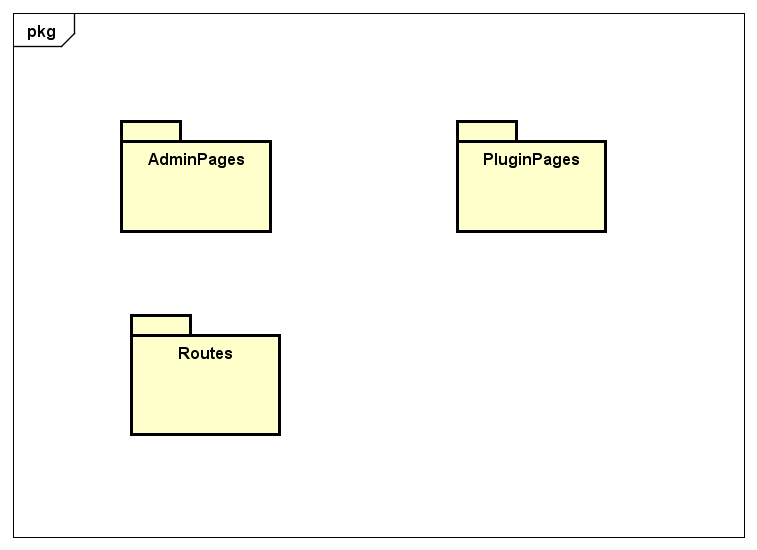
\includegraphics[width=0.8\columnwidth]{prog/pack} 
	\caption{Struttura applicazione}
\end{figure}
\begin{itemize}
	\item \textbf{AdminPages:} contiente tutti i componenti e i servizi\footcite{Nel Appendice si trova una descrizione completa di un servizio Angular} che vanno a formare le pagine(login e di amministratori) per gli utenti di Nextep;
	\item \textbf{PluginPages:} contiene tutti i componenti e i servizi per la pagine contenente l'editor e la pagina contenenti il widget;
	\item \textbf{Routes:} contiene tutto il codice per la gestione della navigazione dell'applicazione.
\end{itemize}
\begin{figure}[!h] 
	\centering 
	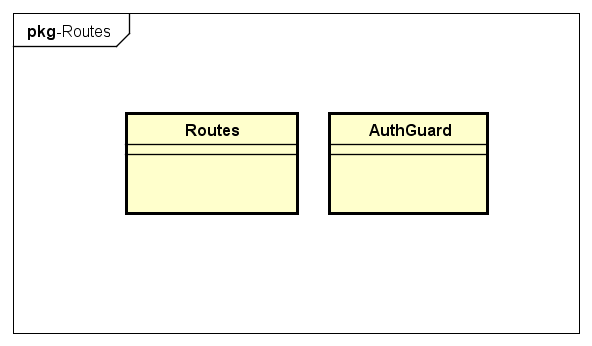
\includegraphics[width=0.6\columnwidth]{prog/routes} 
	\caption{Struttura Routes}
\end{figure}
\begin{itemize}
	\item L'oggetto \textbf{Routes} contiene un array di tutte le navigazioni dell'applicazione,
	\item L'oggetto \textbf{AuthGuard} serve per bloccare la navigazione alla pagina degli amministratori finchè l'utente non effettua il login. 
	\\
\end{itemize}
\subsection{PluginPages}
Contiene tutti i componenti e servizi per realizzare le pagine contenenti l'editor e il widget.
\begin{figure}[!h] 
	\centering 
	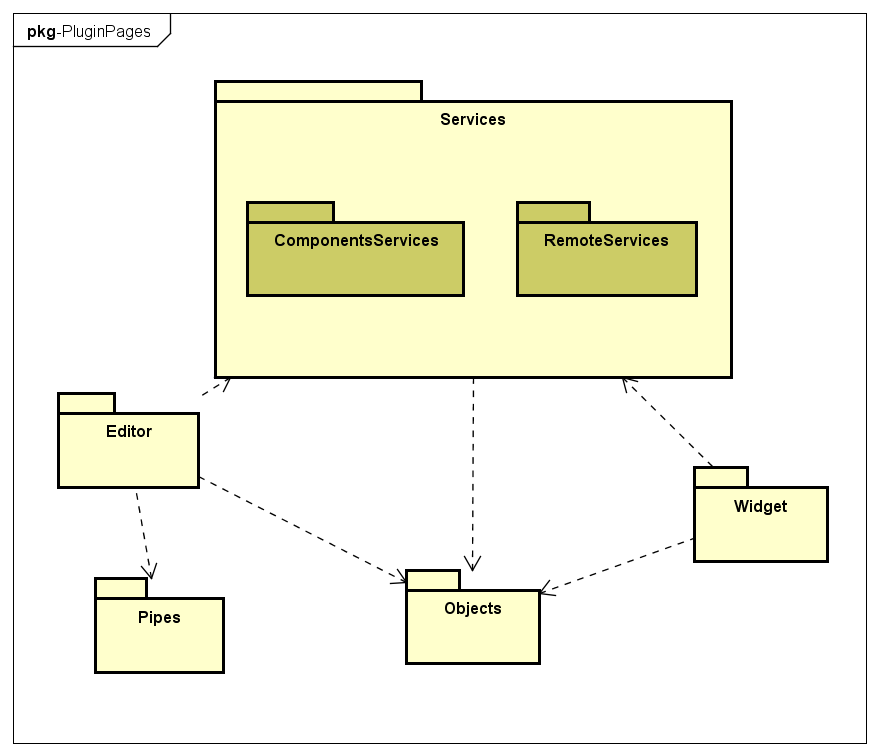
\includegraphics[width=0.8\columnwidth]{prog/pluginpages} 
	\caption{Struttura PluginPages}
\end{figure}
\begin{itemize}
	\item \textbf{ComponentsServices:} contiente tutti i servizi che permettono di scambiare i dati tra i componenti locali;
	\item \textbf{RemoteServices:} contiene tutti i servizi utilizzati per comunicare con il lato backend dell'applicazione. Quindi principalmente per leggere, aggiungere o rimuovere i template dal database su AWS;
	\item \textbf{Objects:} contiene tutti i tipi creati per rappresentare diversi tipi di dati;
	\item \textbf{Editor:} contiene tutti i componenti Angular che formano le pagine contenenti l'editor;
	\item \textbf{Widget:} contiene tutti i componenti Angular che formano le pagina contenenti il widget;
	\item \textbf{Pipes:} contiene le pipes di  Angular.
\end{itemize}
\newpage
\subsection{AdminPages}
Contiene tutti i componenti e servizi per realizzare la pagina di login e la pagina degli amministratori.
\begin{figure}[!h] 
	\centering 
	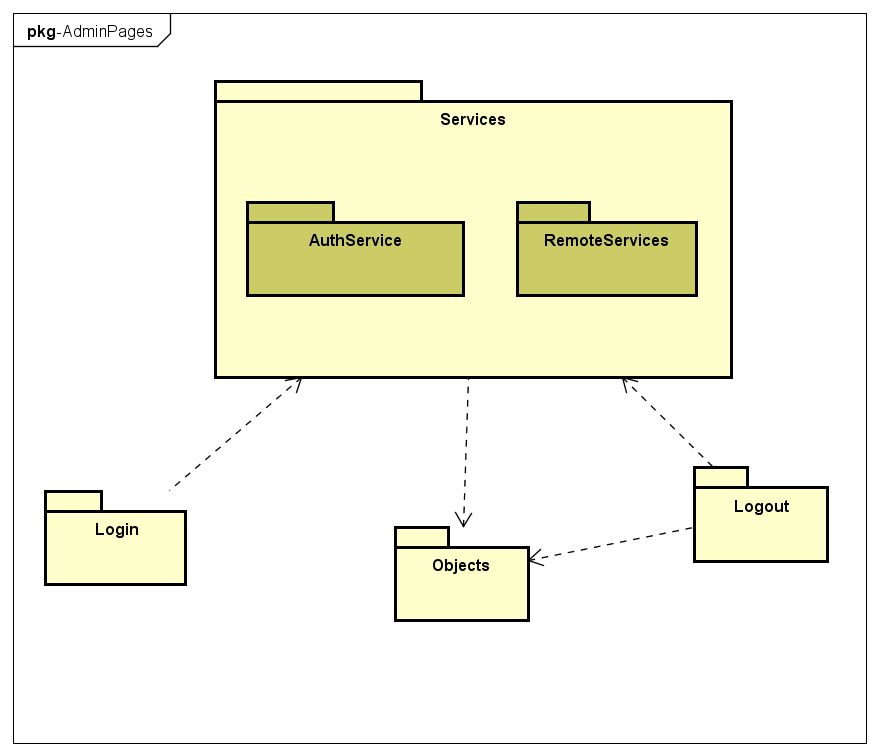
\includegraphics[width=0.8\columnwidth]{prog/adminpages} 
	\caption{Struttura AdminPages}
\end{figure}
\begin{itemize}
	\item \textbf{AuthService:} contiene il servizio che permette di effetuare il login;
	\item \textbf{RemoteServices:} contiene i servizi per aggiungere, leggere o rimuovere i clienti dal database presente su AWS;
	\item \textbf{Objects:} contiene tutti i tipi creati per rappresentare diverse tipologie di dati;
	\item \textbf{Admin:} contiene tutti i componenti Angular che formano la pagina degli amministratori;
	\item \textbf{Login:} contiene tutti i componenti Angular che formano la pagina di login;
\end{itemize}
\subsection{Atomic design}
Per realizzare le diverse pagine dell'applicazione è stato utilizzato il concetto di Atomic Design.
Creata da Brad Frost nel 2013, l'Atomic design è una metodologia composta da 5 differenti fasi, utile per creare un sistema di interfacce in maniera gerarchica. In questa metologia si parte dai componenti piu basilari possibili, fino ad arrivare alle pagine finali. E' quindi un approccio bottom-up.
\begin{figure}[!h] 
	\centering 
	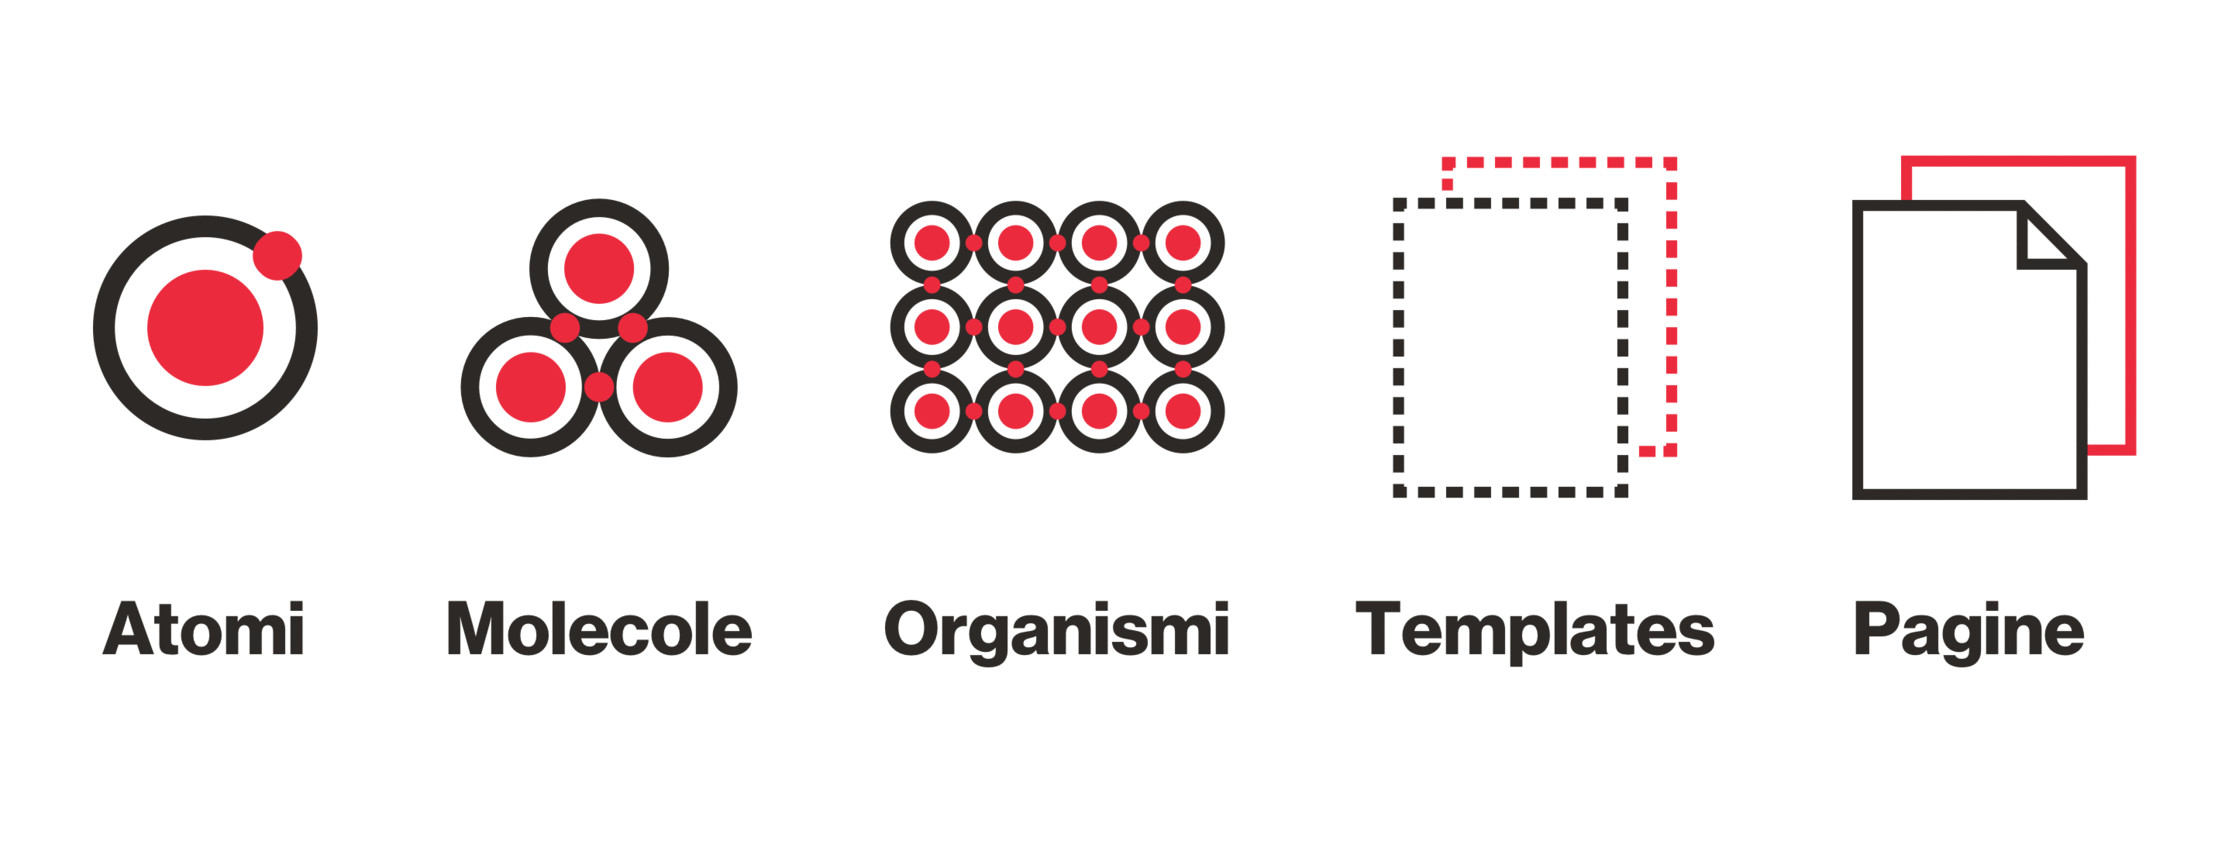
\includegraphics[width=0.8\columnwidth]{atomic} 
	\caption{Elementi atomic design}
\end{figure}
\\

\textbf{Atomi:} in fisica un atomo è la più piccola particella di un elemento che non subisce alterazioni nelle trasformazioni chimiche; nell’Atomic Design gli atomi sono i blocchi fondamentali che comprendono tutta l’interfaccia.
Questi atomi comprendono elementi HTML come tipografia, palette colori, input, bottoni e altri elementi che non possono essere suddivisi ulteriormente senza cessare di essere funzionali.
\\

\textbf{Molecole:} sono semplici gruppi di elementi d'interfaccia che funzionano uniti. Quando combiniamo due oppure più atomi, creiamo quindi una molecola.
\\

Nel contesto dell'applicazione gli atomi e le molecole sono rappresentate dagli elementi della libreria Angular Material, che successivamente sono utilizzati per realizzare l'intera interfaccia dell'applicazione.

\begin{figure}[!h] 
	\centering 
	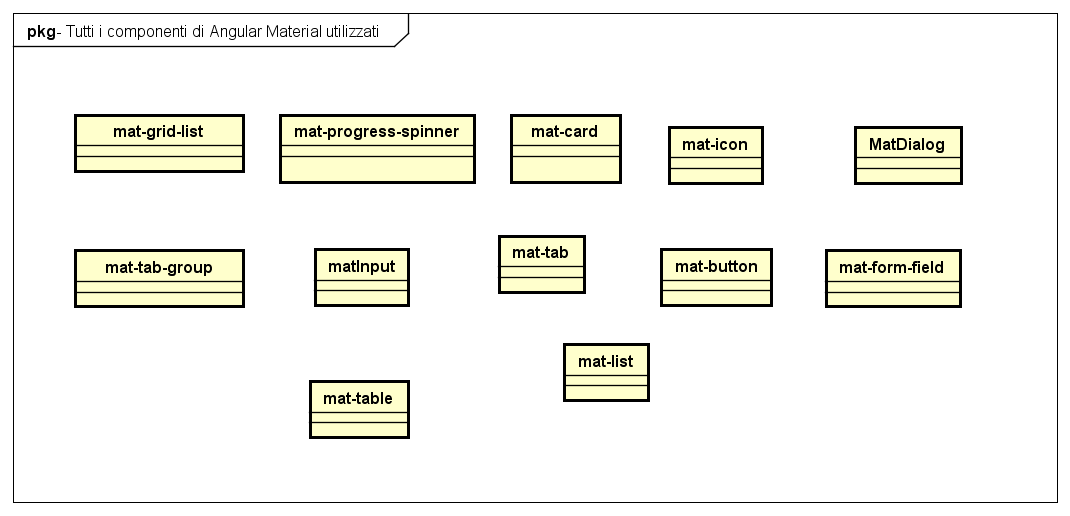
\includegraphics[width=1\columnwidth]{prog/angular} 
	\caption{Componenti Angular Material che formano gli atomi e le molecole dell'applicazione}
\end{figure} 

\textbf{Gli organismi:} sono dei componenti più o meno complessi, composti da gruppi di molecole e/o atomi e/o altri organismi. Questi organismi creano diverse sezioni all'interno della nostra interfaccia. Un esempio può essere un menu di navigazione, che è formato in media da diversi pulsanti/link. 
\\

\textbf{I templates:} sono creati dall'insieme dei nostri atomi, molecole ed organismi creando così la prima idea dello scheletro della pagina.
\\

\textbf{Le pagine:} sono dei templates riempiti di contenuto reale, come immagini, testi, elementi grafici, advertising, ecc. Una pagina quindi è formata da molti template. 
\newpage
\section{Progettazione Backend}
\subsection{Archittetura a microservizi serverless}
Il backend dell'applicazione è realizzato utilizzando i servizi web di Amazon, i servizi scelti sono stati descritti nel capitolo 2. In questa sezione viene descritto come questi servizi comunicano tra di loro. La seguente immagine mostra la panoramica dell'archittettura della applicazione Zendesk realizzata(per la pagina degli amministratori la situazione è leggermente diversa). L'immagine descrive come un template viene caricato nel database NoSQL(database non relazionale) presente su Amazon. 
\begin{figure}[!h] 
	\centering 
	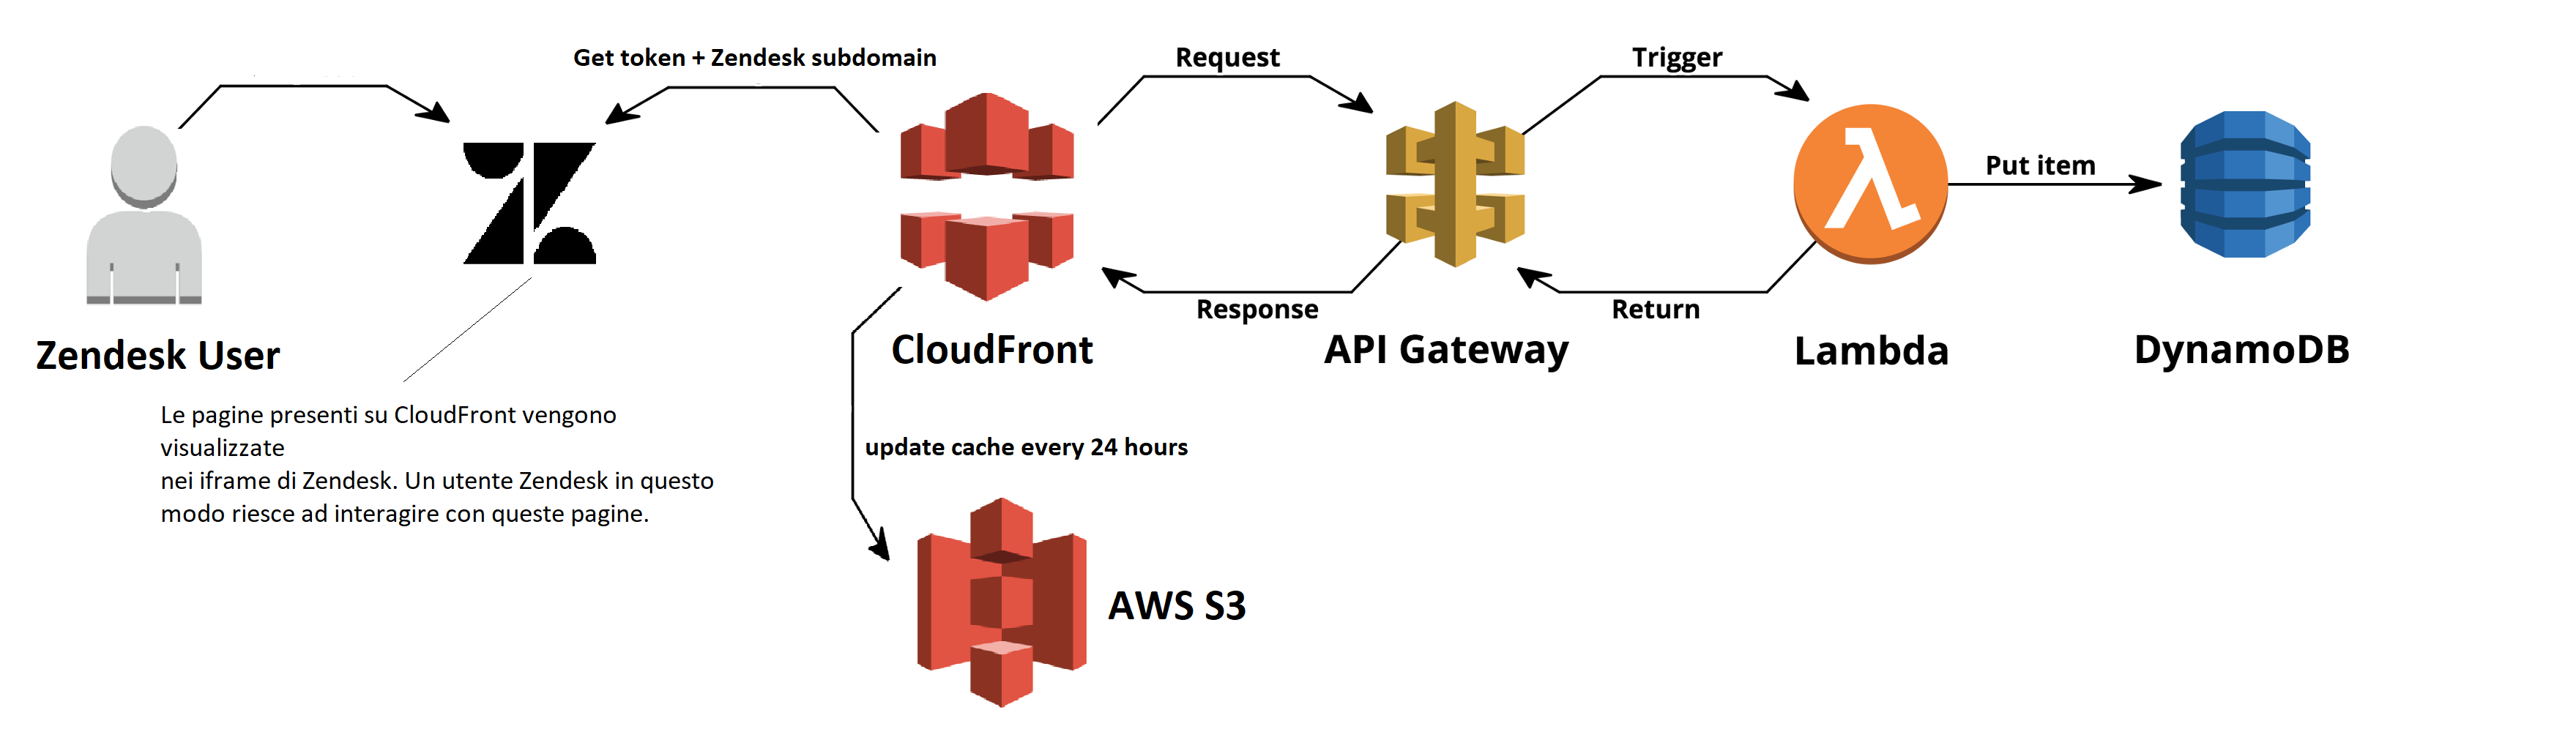
\includegraphics[width=1.2\columnwidth]{prog/zen-architecture} 
	\caption{Flusso completo dell'architettura}
\end{figure} 
\\
\begin{itemize}
	\item Zendesk User interagisce con l'applicazione tramite l'interfaccia di Zendesk;
	\item Le pagine dell'applicazione Angular sono caricate da CloudFront sui iframe presenti su Zendesk;
	\item Le pagine appena caricate nei ifrmae leggono il token e il nome del sottodominio della piattaforma in cui si trovano utilizzando l'oggetto ZAFClient(descritto nel capitolo 2);
	\item Utente crea un nuovo template e lo salva;
	\item L'editor manda la richiesta all'API Gateway inviando nel header il token ed il nome del dominio;
	\item API Gateway come prima cosa verifica il token ed il nome del sottodominio se sono validi. Se sono validi genera un evento che innesca una funzione lambda, altrimenti(token e nomedominio non validi) ritorna un messaggio d'errore;
	\item La funzione lambda riceve dati dall'evento generato da API Gateway. Utilizzando AWS-SDK interagisce con il database nosql e salva il nuovo item(template).
	\item Funzione lambda ritorna un messaggio di successo;
\end{itemize}
\subsection{Archittetura pagina degli amministratori}
Il backend cambia leggermente per quanto riguarda la pagina degli amministratori di Nextep. Per accedere a questa pagina bisogna effettuare il login, il quale è stato implementato utilizzano il servizio Cognito che permette di gestire un pool di utenti in maniera molto semplice. La seguente immagine descrive il funzionamento di questa pagina. 
\begin{figure}[!h] 
	\centering 
	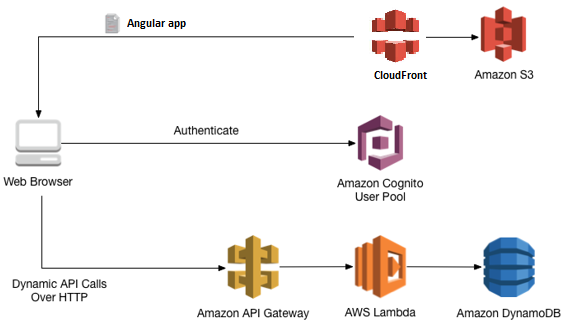
\includegraphics[width=1\columnwidth]{prog/admin-arch} 
	\caption{Flusso completo dell'architettura pagina admin}
\end{figure} 
\begin{itemize}
	\item La pagina di login viene caricata nel browser;
	\item L'utente inserisce le sue credenziali corrette per effettuare il login;
	\item AWS Cognito verifica le credenziali, se sono valide ritorna il token di accesso altrimenti un errore;
	\item Le credenziali sono valide, l'utente accede alla pagina degli amministratori;
	\item L'utente ora può comunicare con l'API Gateway inviando il token ritornato da AWS Cognito. Questo token permette all'utente di inserire oppure eliminare uenti dal database NoSQL presente su AWS;
	\item L'inserimento oppure l'eliminazione di un cliente esegue lo stesso flusso visto sopra per i template. Eccezione fatta per l'AWS Cognito, la pagina degli amministratori ha la stessa architettura.
\end{itemize}
